\documentclass[9pt,twocolumn,twoside]{../../styles/osajnl}
\usepackage{supertabular,booktabs}
\journal{i524} 

\title{Cloudmesh Docker Extension}

\author[1]{Karthick Venkatesan}
\author[2]{Ashok Vuppada}


\affil[1]{School of Informatics and Computing, Bloomington, IN 47408, U.S.A.}


\dates{S17-IR-P009, \today}

\ociscodes{Cloud, I524}

\doi{\url{https://github.com/cloudmesh/sp17-i524/blob/master/project/S17-IR-P009/report/report.pdf}}


\begin{abstract}
Cloudmesh client is a simple client to enable access to multiple cloud environments from a command shell and command line. The users can manage their set of resources right from their workstation.Currently, cloudmesh client supports managing Virtual Machines across multiple clouds. In this project, we have added the capability to manage/provision docker and swarm containers to the cloudmesh client through a simple and extensible command line interface.

\end{abstract}

\setboolean{displaycopyright}{true}

\begin{document}


\maketitle


\section{Introduction}
Docker is an open platform for developing, shipping, and running applications. Docker enables to separate the applications from infrastructure so that we can deliver software quickly. With Docker, one can manage the infrastructure in the same ways we manage our applications\cite{www-Docker}. 

Docker provides the ability to package and run an application in a loosely isolated environment called a container. The isolation and security allow running many containers simultaneously on a given host. Containers are lightweight because they don’t need the extra load of a hypervisor, but run directly within the host machine’s kernel. This means we can run more containers on a given hardware combination than if you were using virtual machines. We can even run Docker containers on host machines that are virtual machines.

Clouldmesh Client\cite{las14cloudmeshmultiple} capability is detailed in Figure~\ref{fig:cmvm},it aims at managing vm instances in multiple heterogeneous clouds remotely via a command line interface.In this project we have added the capability to provision and manage docker\cite{www-Docker} containers  and swarm\cite{www-Swarm} services to cloudmesh client\cite{las14cloudmeshmultiple}.

\begin{figure}[h!]
\centering
\fbox{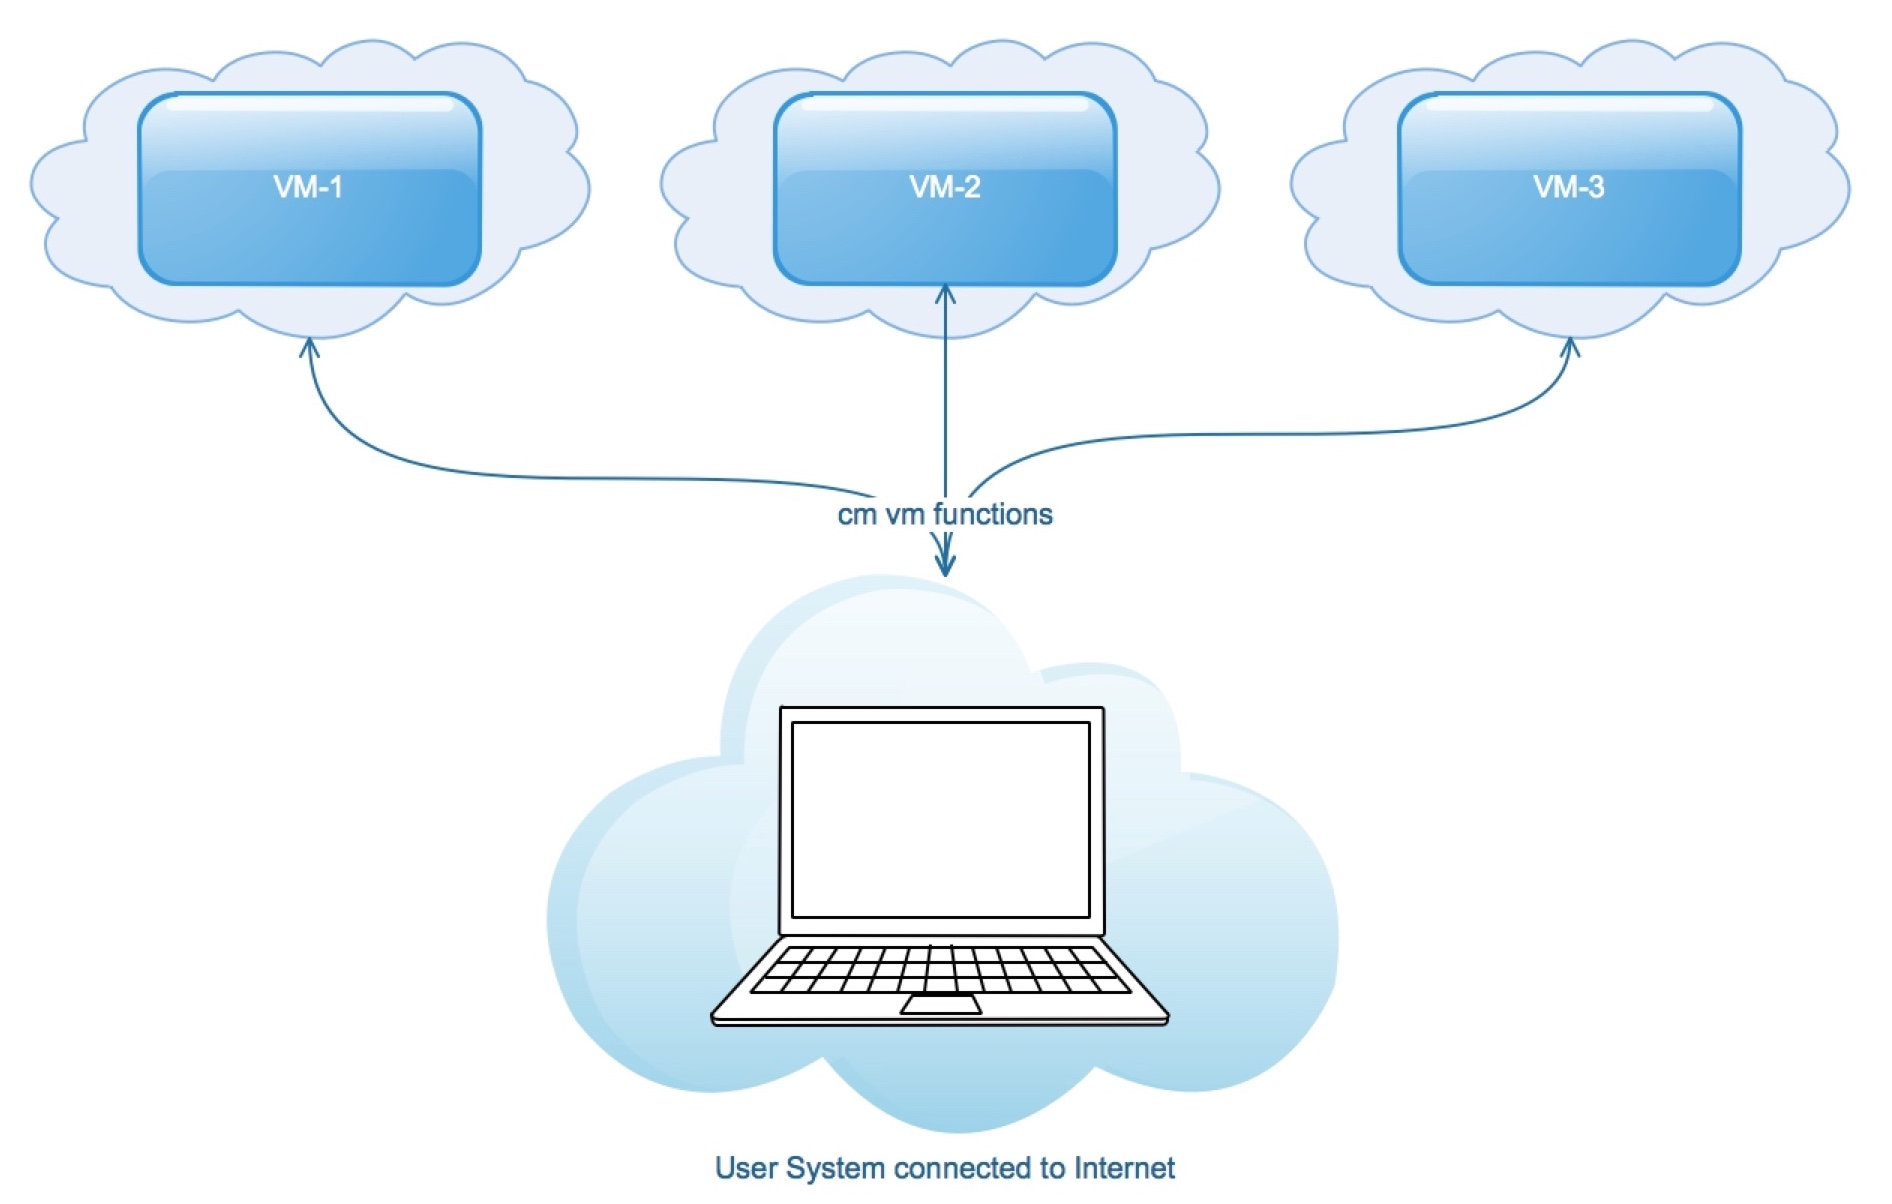
\includegraphics[width=\linewidth]{images/cmvm.jpeg}}
\caption{Cloudmesh client }
\label{fig:cmvm}
\end{figure}


\subsection{Docker Mode}

The key objects of Docker engine are images, containers and networks.An image is a read-only template with instructions for creating a Docker container. A container is a runnable instance of an image.
The Docker Module built in cloudmesh docker application has the capabilities to manage Docker hosts and the underlying objects running on multiple remote VM's as shown in Figure~\ref{fig:cmsdocker}. 

\begin{figure}[h!]
\centering
\fbox{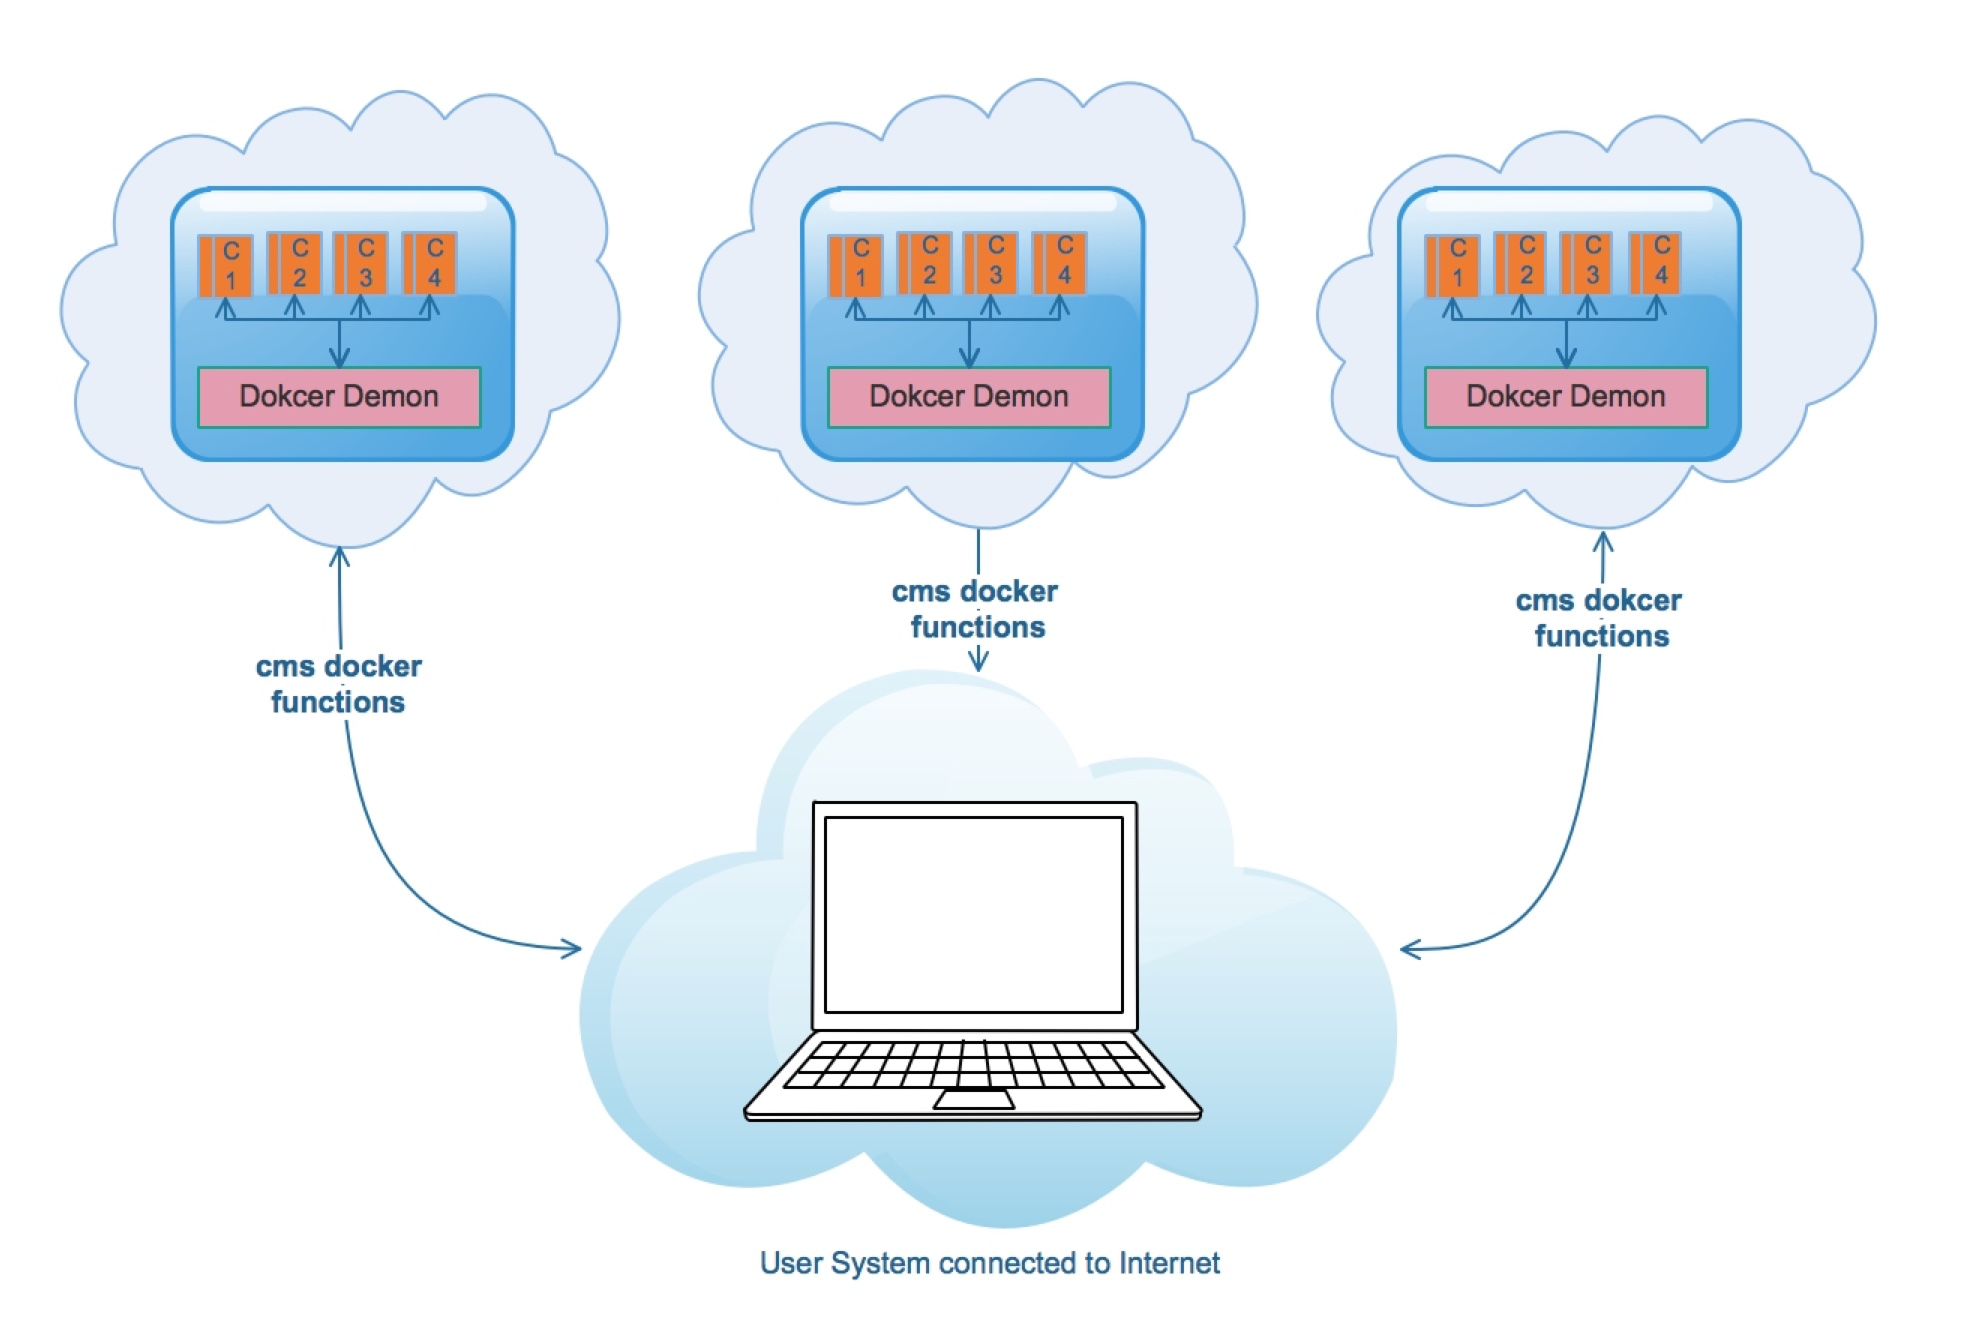
\includegraphics[width=\linewidth]{images/cmsdocker.jpeg}}
\caption{Docker Module }
\label{fig:cmsdocker}
\end{figure}

\subsection{Swarm Mode}

A swarm\cite{www-Swarm} is a cluster of Docker engines, or nodes, participating in a cluster where we deploy services.
The Swarm Mode of Docker orchestrates swarm services in standalone containers on Docker instances.

\subsubsection{Node}
A node is an instance of the Docker Engine participating in the swarm.We can run one or more nodes on a single physical computer or cloud server.

To deploy the application to a swarm, we submit a service definition to a manager node. The manager node dispatches units of work called tasks to worker nodes.

Manager nodes also perform the orchestration and cluster management functions required to maintain the desired state of the swarm. Manager nodes elect a single leader to conduct orchestration tasks.

Worker nodes receive and execute tasks dispatched from manager nodes. By default manager nodes also run services as worker nodes, but we can configure them to run manager tasks exclusively and be manager-only nodes. An agent runs on each worker node and reports on the tasks assigned to it. The worker node notifies the manager node of the current state of its assigned tasks so that the manager can maintain the desired state of each worker.


\subsubsection{Services and Tasks}

A service is the definition of the tasks to execute on the worker nodes. It is the central structure of the swarm system and the primary root of user interaction with the swarm.When we create a service, we specify which container image to use and which commands to execute inside running containers.

In the replicated services model, the swarm manager distributes a specific number of replica tasks among the nodes based upon the scale we set in the desired state.

For global services, the swarm runs one task for the service on every available node in the cluster.

A task carries a Docker container and the commands to run inside the container. It is the atomic scheduling unit of swarm. Manager nodes assign tasks to worker nodes according to the number of replicas set in the service scale. Once a task is assigned to a node, it cannot move to another node. It can only run on the assigned node or fail.


\begin{figure}[h!]
\centering
\fbox{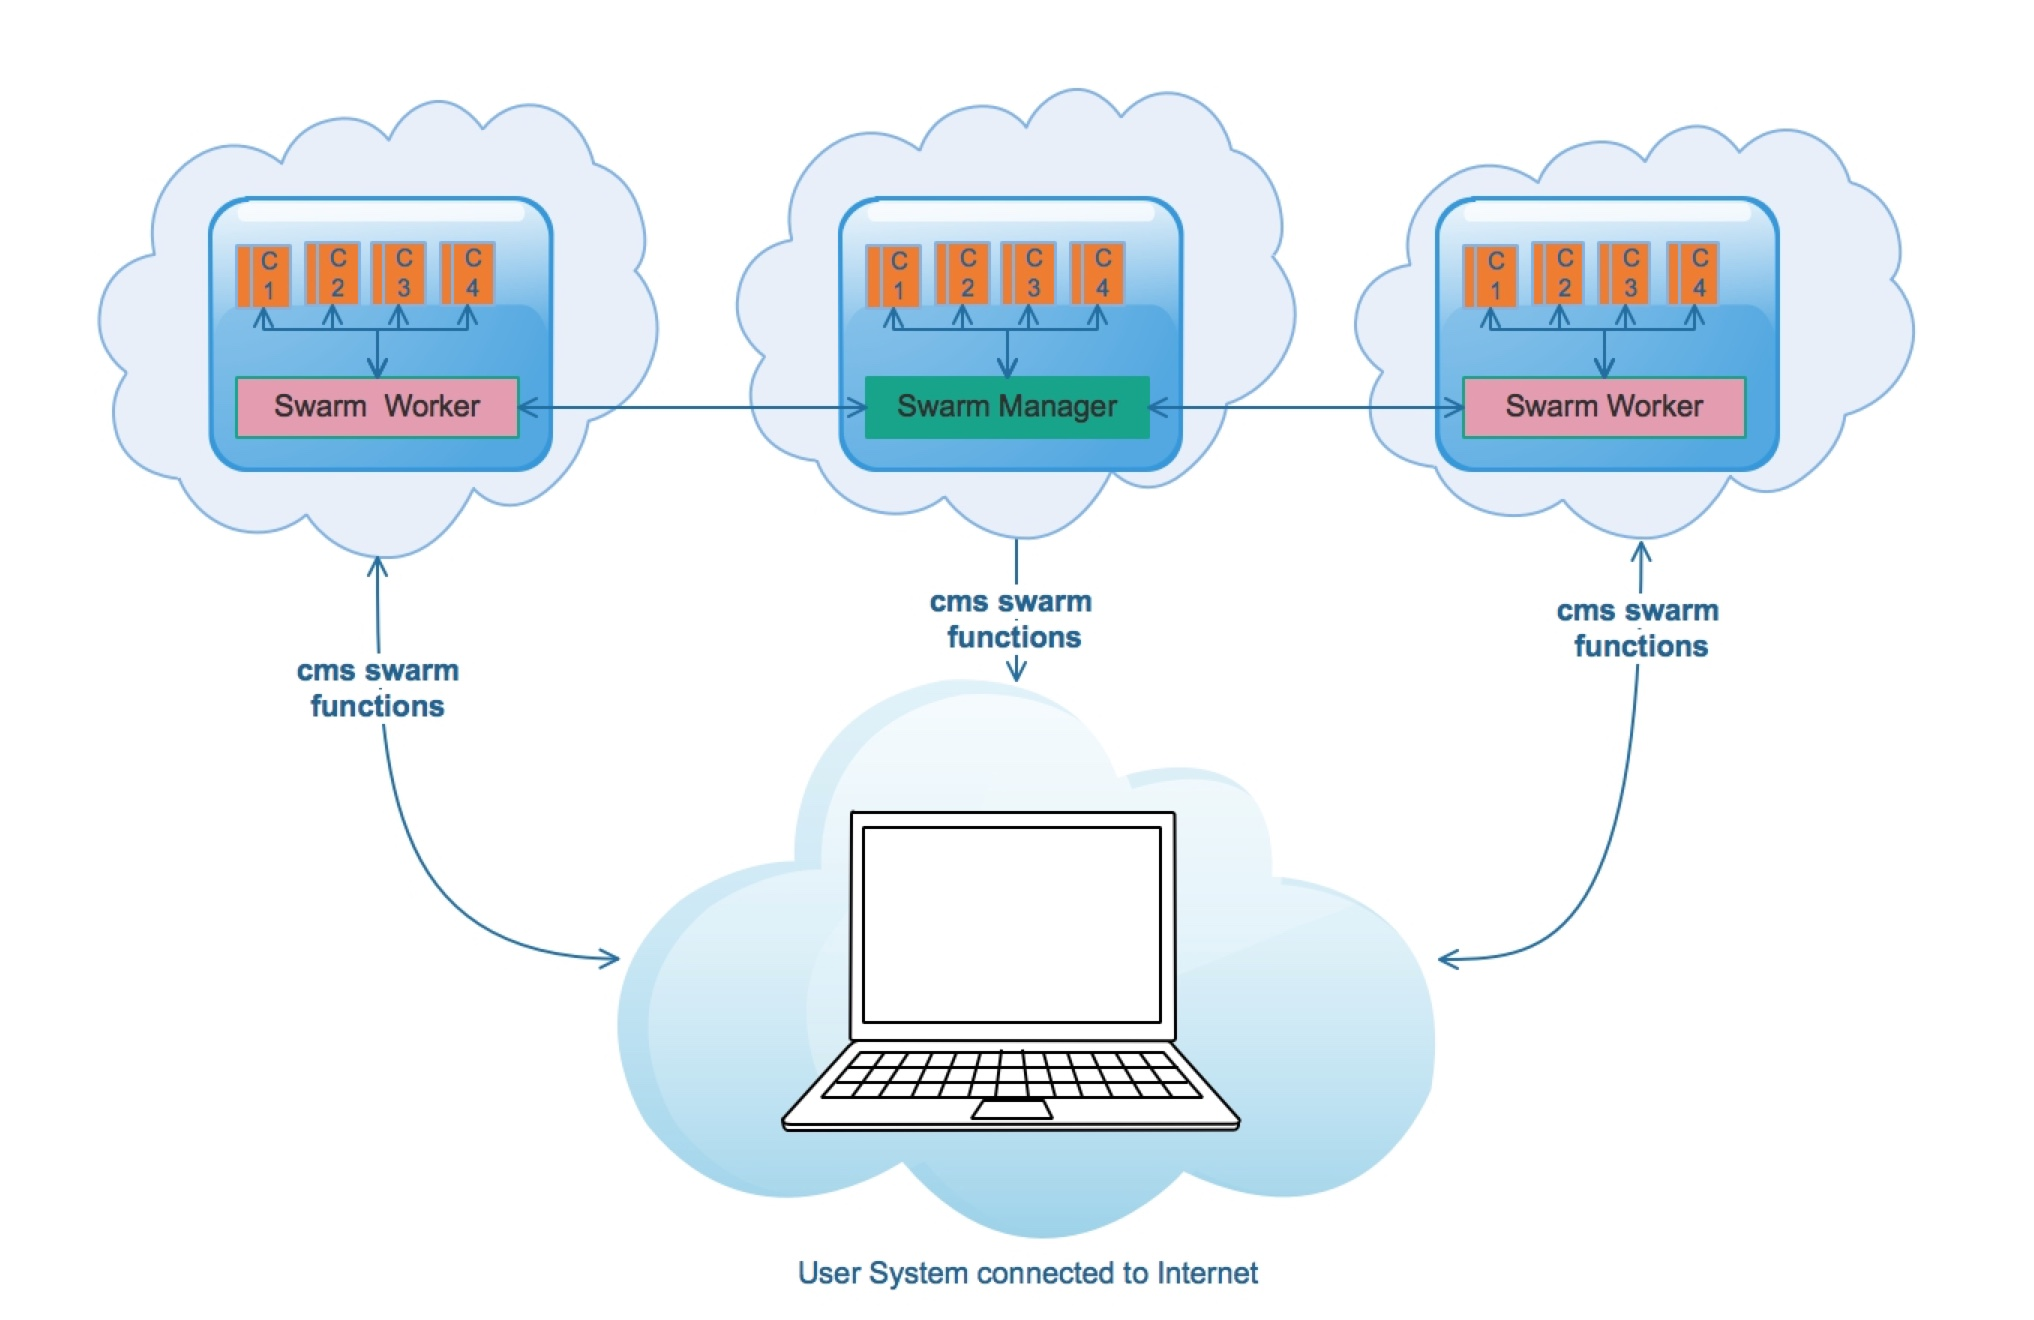
\includegraphics[width=\linewidth]{images/cmsswarm.jpeg}}
\caption{Swarm Module }
\label{fig:cmsswarm}
\end{figure}

The Swarm Module built in cloudmesh.Docker application has the capabilities to create and manage a swarm cluster running of multiple remote VM's as shown in Figure~\ref{fig:cmsswarm}. 
\subsection{Remote vs Local use}
Users can choose to use cloudmesh docker application from a remote terminal outside the network of the data centre as in Figure~\ref{fig:cmsdocker} or locally from a provisioning or configuration server inside the data centre as in Figure~\ref{fig:cmsdocker-2}.We have analysed this difference in the application usage in depth in the project and have provided detailed benchmark results for both modes of use.
\begin{figure}[h!]
\centering
\fbox{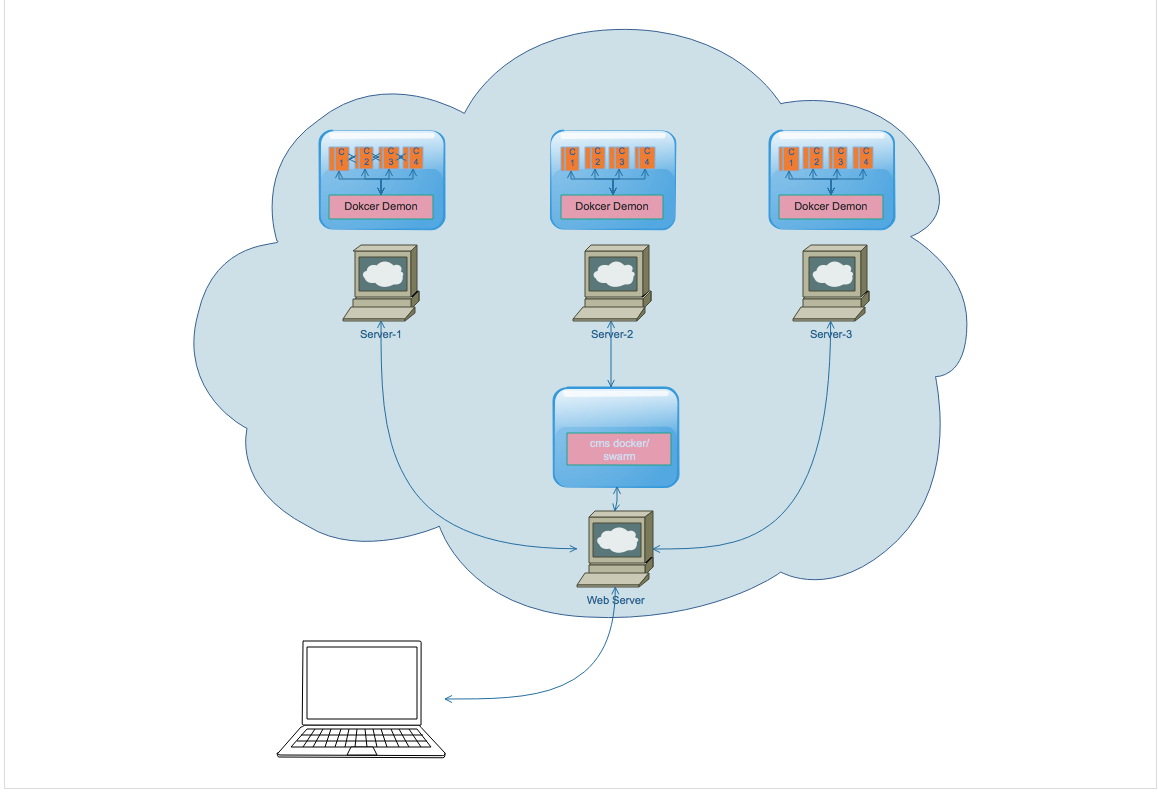
\includegraphics[width=\linewidth]{images/cmsdocker-2.png}}
\caption{Docker/Swarm Remote }
\label{fig:cmsdocker-2}
\end{figure}



\section{Cloudmesh Docker Application Architecture}
The architecture of the application is depicted in Figure~\ref{fig:Arch}.The commands developed can be broadly classified as 'action commands','Inquiry commands'.\\
The action commands are which would create or alter an entity.The entity can be a host/container/node. We use the corresponding API call to get the latest values for the changed entity.Docker API module is developed for addressing the docker commands, and Swarm API module is used for swarm commands.
The Inquiry commands have two flavours a list and refresh mode.The list commands fetch the data locally from the Database and the refresh command will refresh the current state of the corresponding entity from the hosts.

\subsection{Technologies Used}
\begin{table}[H]
\centering
\begin{tabular}{|cp{3cm}|} 
 \hline
 Name & Purpose \\ 
 \hline
 docker \cite{www-Docker} & Docker Server and Api for managing containers and services \\ 
 mongodb \cite{www-MongoDB} & Nosql DBMS \\ 
 Python-eve    \cite{www-Pythoneve} & Restful webservices interface to mongoDB \\ 
 python \cite{www-Python} & Development  \\ 
 ansible \cite{www-Ansible} & Automated deployment \\ [1ex] 
\hline
\end{tabular}
\caption{Technology Name and Purpose}
\label{table:1}
\end{table}

\subsection{MongoDB and Python-eve}

The cloudmesh docker application uses MongoDB\cite{www-MongoDB} for data storage.The access to the database is all through
restful services supported through Python-eve\cite{www-Pythoneve}.The following are the entities for which collections are defined in Eve and MongoDB.

\begin{enumerate}
\item Host
\item Image
\item Container
\item Network
\item Service
\item Node
\end{enumerate}
A key benefit of using a NoSQL database like MongoDB is that it allowed us to store the data in the DB in the native form as returned by the Docker API without the need for much marshalling of the data.

\begin{figure}[htbp]
\centering
\fbox{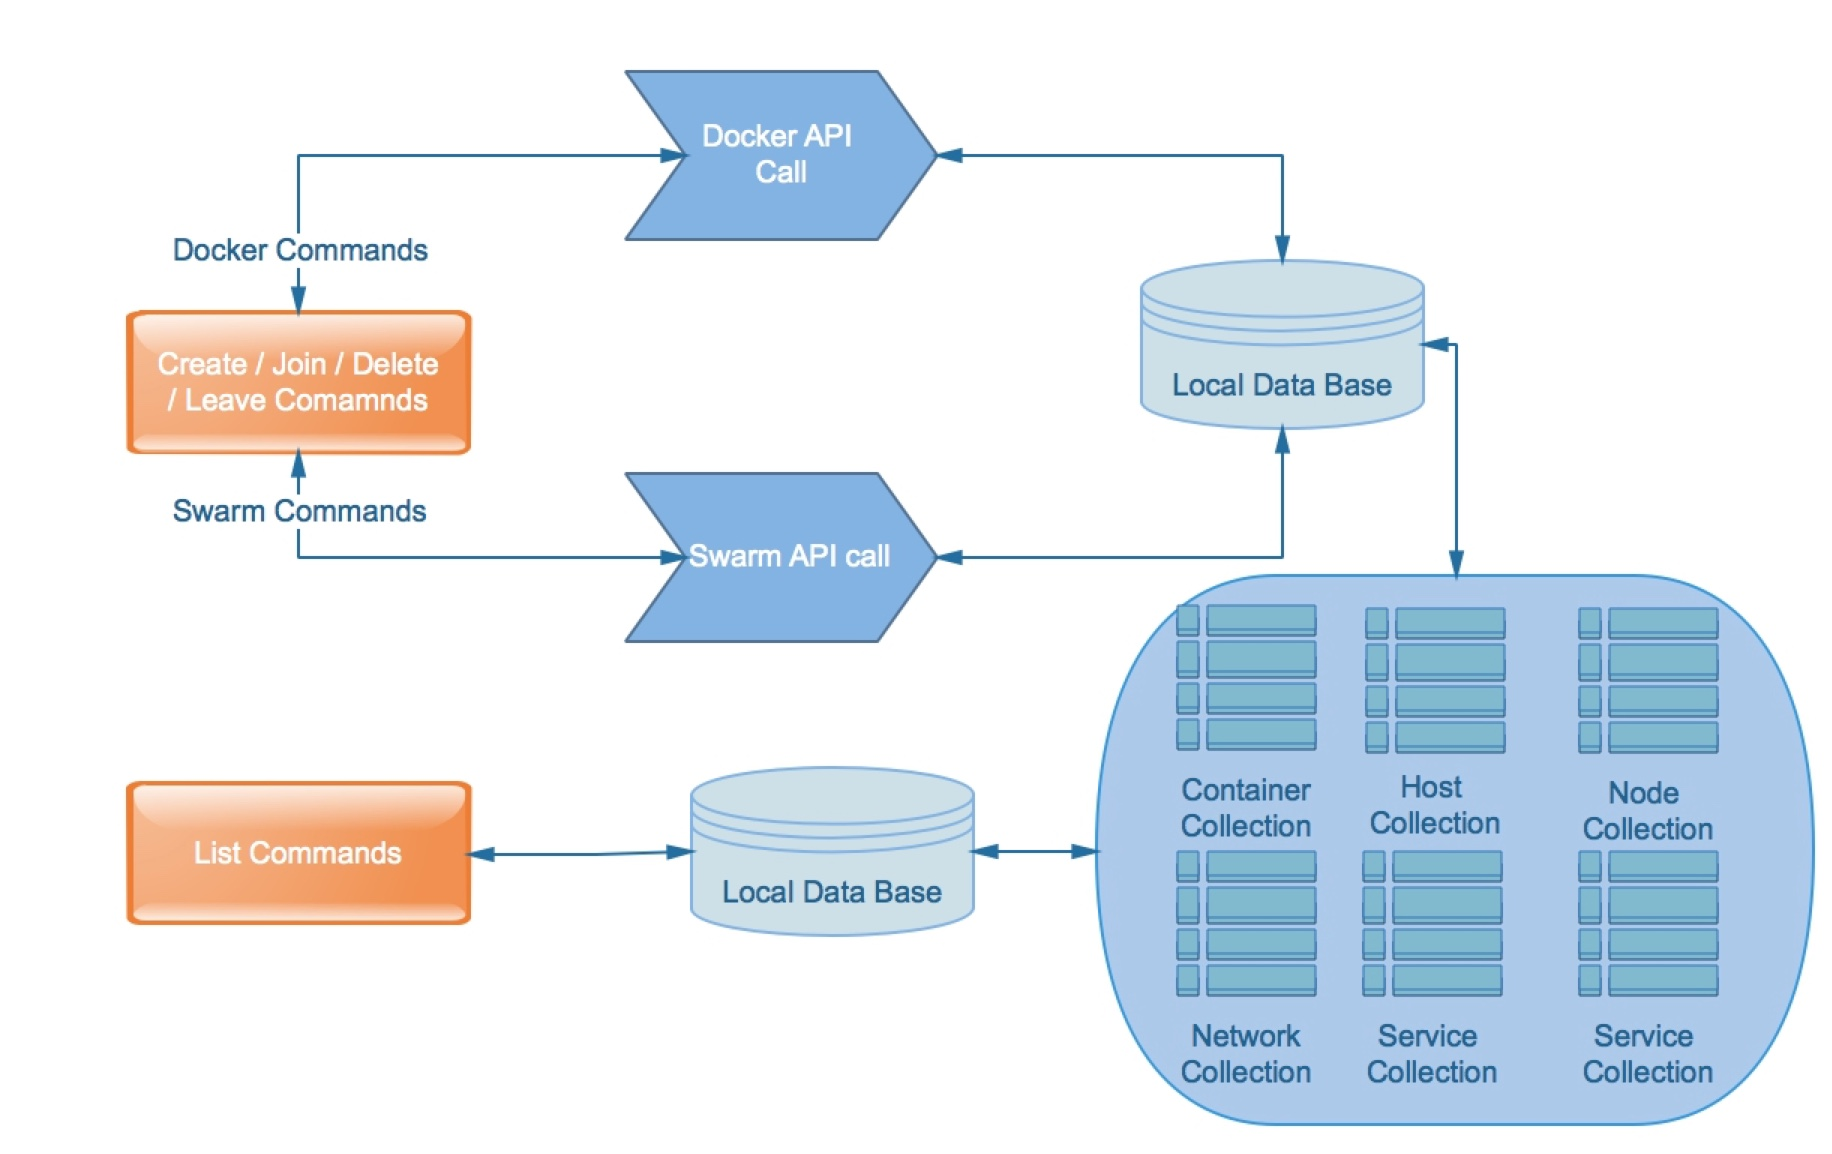
\includegraphics[width=\linewidth]{images/Arch.jpeg}}
\caption{cloudmesh docker application architecture}
\label{fig:Arch}
\end{figure}

\subsection{Security}

We have not yet fully baked in security aspects into the client.We propose that security between the various aspects of the application will be handled as below

\begin{enumerate}
\item The docker daemon on the remote Hosts / VM are to be exposed to be accessed by cloudmesh Docker application.We envision that there would be separate configuration machines either within the network of the user's infrastructure or outside which will have a secure access.The docker daemons will be configured to accept connections only from this remote host.Alternatively, if there are multiple configuration machines, then specific security groups need to created between the client machine and each docker host for secure access.

\item The Python-eve client currently runs on a local machine and will accept connections only from the localhost from were the client is run.We also envision adding a user access control to the Python-eve services which will facilitate making the service and the Mongo DB to be deployed on a remote central server different from the client and allowing only authenticated users to use the application.
 \end{enumerate}

\subsection{Cloudmesh Common}

The application makes extensive use of common functions and tightly integrated into common functions available in the cloudmesh common repository for display formatting, YAML config management and timers

\subsection{Ansible}

As part of the project we have built Ansible\cite{www-Ansible} scripts to automate the installation of Docker in remote hosts and also deployment of Docker images in these remote docker hosts.Below is the list of Ansible scripts that are built and used in the project 
\begin{enumerate}
\item Install Docker in remote hosts and enable them for remote API access
\item Install Docker images in Docker hosts.As part of the script, the local docker files are synced with remote hosts, and the images are built.
\item Setup /etc/hosts for remote hosts.This script allows to setup host names in remote hosts which allow the applications running on these hosts to be configured to access other applications on the network by the standard host names instead of the IP address.
\end{enumerate}

\subsection{Project Repository}

The source code and the detailed deployment and use instructions are available at \cite{github-Cloudmesh-Docker} 
\section{Docker Commands}
\begin{enumerate}
    \item\textbf{Host Set/Add}
     This command will Set/Add the docker host on which the user wants to operate.The host details will be captured in the database with this command.
    \begin{verbatim} cms docker host docker1 docker1:4243 \end{verbatim}
    
    \item \textbf{Host List}
     This command will list the hosts available.The output would display the Ip, Name, Port,and if the host is swarm manager and the swarm manager Ip. Please note the Swarm manager Ip will be blank if the host is manager or not part of swarm. 
     \begin{verbatim}
     cms docker host list 
     \end{verbatim}
     
     \begin{table}[h!]
     \caption{\bf cms docker host list }
     \begin{tabular}{ccccc}
     \hline
      Ip & Name & port & Swarmmode &SwarmManagerIp\\
      \hline
      docker1 & docker1 & 4243 & Manager & \\
      docker2 & docker2 & 4243 & Worker & docker1\\
      docker3 & docker1 & 4243 & Host & \\
     \hline
     \end{tabular}
     \label{tab:tab1}
     \end{table}
     
    \item \textbf{Host Delete}
    This command will delete the host from the setup.This would also delete the host details from the database.User can do a host list to see the updated host details.\\
    \begin{verbatim}
    cms docker host delete docker1:4243
    \end{verbatim}
    
    \item \textbf{Image List}
    This command will display the images available on the hosts available in the database.
    It would display the Ip of the host, the Image Id, repository and the size of the image.Please note that this command would display the results from the local dB.\\
    \begin{verbatim}
    cms docker image list
    \end{verbatim}
    
    \begin{table}[h!]
     \caption{\bf cms docker image list }
     \begin{tabular}{cccc}
     \hline
      Ip & Id & Repository & Size(GB)\\
      \hline
      docker1 & 5545f4e3b27e & cloudmesh:docker & 5.59 \\
      docker2 & 45f4e3b2799e & elasticsearch:swarm & 0.45 \\
     \hline
     \end{tabular}
     \label{tab:tab2}
     \end{table}
     
    \item \textbf{Image Refresh} 
     This command would refresh the images across the hosts available. The results are updated to the local data base.
    \begin{verbatim}
    cms docker image refresh
    \end{verbatim}

    \item \textbf{Container Create}
     This command will create a container on a given host.The arguments for this command is the name of the container and the image from which the container needs to be created.The image in the argument must be available through image list command above on the given host.\\
 
    \begin{verbatim}
    cms docker container create test1 \
    elasticsearch:docker
    \end{verbatim}
    
    \item \textbf{Container Start}
     This command will start a container.The container should have been already created using the create command.\\

    \begin{verbatim}
    cms docker container start test1
    \end{verbatim}     
     
    \item \textbf{Container Stop}
     This command will stop and container which is running.\\

    \begin{verbatim}
    cms docker container stop test1
    \end{verbatim}  
    
    \item \textbf{Container List}
     This command will display the list of containers running across the hosts.The output contains the Ip, Container Id, Name, Image, status and start time of the container.The details would be shown from the local database maintained.
     
    \begin{verbatim}
    cms docker container list
    \end{verbatim}  
        
     \begin{table}[h!]
     \caption{\bf cms docker container list }
     \begin{tabular}{cccccc}
     \hline
      Ip & Id & Name & Image &Status&StartedAt\\
      \hline
      docker1 & 5545f4e3b27e & test1 & image1 &exited & 12.00PM \\
     \hline
     \end{tabular}
     \label{tab:tab3}
     \end{table}
     
    \item \textbf{Container Refresh}
     This command will refresh the current state of the containers across the hosts. This application will connect to all the hosts available in the database and run the native Docker container list to get the latest information and update the local database for refreshing the data. \\
     
    \begin{verbatim}
    cms docker container refresh
    \end{verbatim}  
    
    \item \textbf{Container Delete}
     This command will delete the container on the host. The argument required is the container name.The updated container list can be viewed by running cms docker container list command.\\
     
    \begin{verbatim}
    cms docker container delete test1 
    \end{verbatim}  
    
    
    \item \textbf{Container Run}
     This command will create and run a container in one step.The arguments for the function are the name of the container and the image from which it needs to be run.\\
     
    \begin{verbatim}
    cms docker container run test1 /
    elasticsearch:docker
    \end{verbatim}  

    \item \textbf{Container Pause}
     This command will pause the container which is currently running.\\
     
    \begin{verbatim}
    cms docker container pause test1
    \end{verbatim} 

    \item \textbf{Container Unpause}
     This command will unpause the container which is currently paused.
     
    \begin{verbatim}
    cms docker container unpause test1
    \end{verbatim} 

    \item \textbf{Network Refresh}
    This command will refresh the network details across all the available hosts in the database and  update the results to the local database.
    
    \begin{verbatim}
    cms docker network refresh
    \end{verbatim} 

    \item \textbf{Network List}
    This command will display the network details available in the local database.The output would display the host Ip where the network is established, the network Id , name and containers on the network\\

    \begin{verbatim}
    cms docker network list
    \end{verbatim} 
    
    \begin{table}[htbp]
     \caption{\bf cms docker network list }
     \begin{tabular}{cccc}
     \hline
      Ip & Id & Name & Containers\\
      \hline
      docker1 & 5545f4e3b27e & network1 & test1  \\
     \hline
     \end{tabular}
     \label{tab:tab4}
     \end{table}
\end{enumerate}


\section{Swarm Commands}
\begin{enumerate}
    \item \textbf{Host Set/Add}
     The command will add or set the input host to the current host.The swarm commands following this command will be executed on the host setup in this step. The host details will also be captured in the database as part of this command.\\
     
    \begin{verbatim}
    cms swarm host docker1 docker1:4243
    \end{verbatim} 

     
    \item \textbf{Host List}
     This command will list the hosts available. It displays the Ip, Name,Port,and if the host is swarm manager and the swarm manager Ip. Please note the Swarm manager Ip will be blank if the host is manager or not part of swarm.
     
    \begin{verbatim}
    cms swarm host list
    \end{verbatim} 

     \begin{table}[htbp]
     \caption{\bf cms docker host list }
     \begin{tabular}{ccccc}
     \hline
      Ip & Name & port & Swarmmode &SwarmManagerIp\\
      \hline
      docker1 & docker1 & 4243 & Manager & \\
      docker2 & docker2 & 4243 & Worker & docker1\\
      docker3 & docker1 & 4243 & Host & \\
     \hline
     \end{tabular}
     \label{tab:tab5}
     \end{table}
     
    \item \textbf{Host Delete}
    This command will delete the host from the database and also the associate container,service,networkand image objects of the host.\\

    \begin{verbatim}
    cms swarm host delete docker1:4243
    \end{verbatim} 
    
    \item \textbf{Image List}
    This command will display the images available on a host.
    It would display the Ip of the host, the Image Id , repository and the size of the image.Please note that this command would display the results from the local dB.\\
    
    \begin{verbatim}
    cms swarm Image list
    \end{verbatim} 

    
    \item \textbf{Swarm Create}
    This command will initialise the  swarm mode on the current host.There are no arguments required for this command. After this command is run the current host would become the swarm manager.\\
    
    \begin{verbatim}
    cms swarm create
    \end{verbatim} 
    
    \item \textbf{Swarm Join}
    This command will join the current host to a swarm node either as a manager or a worker. User needs to setup a new current host with cms swarm host command and run cms swarm join so that current host would be joined with the swarm created.User needs to pass the address or host name of the swarm manager and the mode in which the current node will operate in the swarm.\\
    
    \begin{verbatim}
    cms swarm join docker3 docker4:4243 worker
    \end{verbatim} 
    ( assuming docker3 is already a swarm manager) 
    
    \item \textbf{Swarm Leave}
    This command is applicable for the swarm manager or worker, this would remove the host from the swarm.If a manager has multiple workers, workers need to be removed(leave) before the manager can leave.\\
    
    \begin{verbatim}
    cms swarm leave 
    \end{verbatim}

    
    \item \textbf{Network Create}
    This command will create the network which can be used by the swarm containers later.The argument it needs is the name of the containers.
    
    \begin{verbatim}
    cms swarm network create network1 
    \end{verbatim}
    
    \item \textbf{Network List}
     This command will display the network details from the local database.The output will display the host Ip where the network is established, the network Id, name and containers on the network\\
     
    \begin{verbatim}
    cms swarm network list  
    \end{verbatim}
    
    \begin{table}[htbp]
     \caption{\bf cms swarm network list }
     \begin{tabular}{cccc}
     \hline
      Ip & Id & Name & Containers\\
      \hline
      docker1 & 5545f4e3b27e & network1 & test1  \\
     \hline
     \end{tabular}
     \label{tab:tab6}
     \end{table}
     
    \item \textbf{Network Refresh}
    This command will refresh the network details across the Docker hosts available in the database and update the results in the local database.\\
    
    \begin{verbatim}
    cms swarm network refresh  
    \end{verbatim}
    
    
    \item \textbf{Network Delete}
    This command will delete an existing network.The input required for this command is just the network name.
    
    \begin{verbatim}
    cms swarm network delete network1  
    \end{verbatim}
    
    
    \item \textbf{Service Create}
    This command will create a service, the arguments required are the image name and the name of service.This command will record the service details into the local database.This command also takes several configurable options such as Replica Count , Replica Mode and Network which can be passed as advanced options as detailed in Section 5.\\
    
    \begin{verbatim}
    cms swarm service create elasticsearch \
    elasticsearch:swarm  
    \end{verbatim}
    
    \item \textbf{Service List}
    This command will list the current services running , the data displayed is from the local database, if the most current details are required user can run service refresh command below.\\

    \begin{verbatim}
    cms swarm service list 
    \end{verbatim}  
    
    The number of replicas below indicates the number of containers which are running the services.\\
    \begin{table}[htbp]
     \caption{\bf cms swarm service list }
     \begin{tabular}{p{1.25cm}p{1.5cm}p{1.5cm}p{1.5cm}p{.75cm}}
     \hline
      Ip & Id & Name &Image & Replicas\\
      \hline
      docker1 & 5545f4e3b27e & elasticsearch &elastic:swarm  & 3  \\
     \hline
     \end{tabular}
     \label{tab:tab7}
     \end{table}
     
    \item \textbf{Service Delete}
    This command will delete a running service, the argument required is the service name.This command will also delete the service details into the local database.\\
    
    \begin{verbatim}
    cms swarm service delete elasticsearch
    \end{verbatim} 
    
    \item \textbf{Service Refresh}
    This command will refresh the services status for all the hosts available in the database and refresh the service details in the local database.
 
    \begin{verbatim}
    cms swarm service refresh
    \end{verbatim} 
       
    \item \textbf{Node List}
    This command will display the list of the nodes across the hosts available.The results come from the local database. The command will display the node Id, node Ip, Role, Status and Manager Ip.
    
    \begin{verbatim}
    cms swarm node list
    \end{verbatim} 

     \begin{table}[htbp]
     \caption{\bf cms swarm node list }
     \begin{tabular}{ccccc}
     \hline
      Id & Ip & Role &Status & Manager Ip\\
      \hline
      5545f4e3b27e &docker3& Manager&Ready&  \\
      7645f4f4b27e &docker2& Worker&Ready&docker4  \\
     \hline
     \end{tabular}
     \label{tab:tab8}
     \end{table}
     
    \item \textbf{Image Refresh}
    This command will refresh the images details across the hosts available in the database and store the results in the local database .
    
    \begin{verbatim}
    cms swarm image refresh
    \end{verbatim} 
     
    \item \textbf{Image List}
    This command will display the images available on a host.
    It would display the Ip of the host, the Image Id, repository and the size of the image.Please note that this command would display the results from the local dB.\\
    
    \begin{verbatim}
    cms swarm image list
    \end{verbatim} 
    
    \begin{table}[htbp]
     \caption{\bf cms swarm image list }
     \begin{tabular}{cccc}
     \hline
      Ip & Id & Repository & Size(GB)\\
      \hline
      docker1 & 5545f4e3b27e & cloudmesh:docker & 5.59 \\
      docker2 & 45f4e3b2799e & elasticsearch:swarm & 0.45 \\
     \hline
     \end{tabular}
     \label{tab:tab9}
     \end{table}
     
    \item \textbf{Container Refresh}
    This command will refresh the current state of the containers across the hosts available in the local database. This command would connect to the host and run the native Docker container list to get the latest information and update the local database  refreshing the data. \\
    
    \begin{verbatim}
    cms swarm container refresh
    \end{verbatim} 

    \item \textbf{Container List}
    This command will display the list of containers running across the hosts.This would return the Ip, Container Id, Name, Image, status and start time of the container.The details would be shown from the local database maintained.
    
    \begin{verbatim}
    cms swarm container list
    \end{verbatim} 
    
     \begin{table}[htbp]
     \caption{\bf container list }
     \begin{tabular}{cccccc}
     \hline
      Ip & Id & Name & Image &Status&StartedAt\\
      \hline
      docker1 & 5545f4e3b27e & test1 & image1 &exited & 12.00PM \\
     \hline
     \end{tabular}
     \label{tab:tab10}
     \end{table}
\end{enumerate}

 \section{Docker and Swarm Commands Advanced Options}

All the commands in the docker and the swarm module support optional advanced parameters that allow customising the docker containers, services and networks that are created.A detailed list of these arguments is available at \cite{Docker-Python-SDK}.The advanced options can be added to commands as simple name value pairs.

\section{Use Case - Elasticsearch cluster }
 Elasticsearch\cite{www-ElasticSearch} is an open-source, broadly-distributable, readily-scalable, enterprise-grade search engine. Accessible through an extensive and elaborate API, Elasticsearch can power extremely fast searches that support your data discovery applications[2]

 Using Cloudmesh  client, Ansible and Cloudmesh Docker application we deployed and provisioned an Elasticsearch cluster on remote hosts in Chameleon cloud in Docker and swarm mode.We benchmarked the cluster using esrally\cite{www-ElasticSearchRally}  have compared the results between the elastic search clusters in Docker and swarm mode.


The hardware specifications used on both the clouds is detailed in Table~\ref{tab:eshardware}

\begin{table}[h]
\centering
\caption{Deployment Hardware Specification}
\label{tab:eshardware}
\begin{tabular}{|l|l|l|}
\hline
 & \textbf{Chameleon} & \textbf{Aws} \\ \hline
\textbf{VM} & 3 & 3 \\
\textbf{Containers} & 5 & 5 \\
\textbf{OS} & Ubuntu 16.04 & Ubuntu 16.04 \\
\textbf{Flavor} & m1.large & t2.large \\
\textbf{VCPU} & 4 & 2 \\
\textbf{Memory} & 8 GB & 8 GB \\
\textbf{Storage} & 80 GB & 80 GB\\
\hline
\end{tabular}
\end{table}
 


 \subsection{Elasticsearch Cluster Docker Mode}
  For provisioning, the Elasticsearch cluster in Docker hosts below are the steps done
\begin{enumerate}
\item Created 3 Virtual Machines using Cloud Mesh Client .2 of the Virtual Machines  are to be used for the docker Elasticsearch cluster, and 1 Virtual machine is the Benchmark server for the Kibana and esrally docker images 
\item Using Ansible scripts Install Docker in 3 Virtual Machines and enable the docker daemon for remote access.
\item Using Ansible scripts Install Images of Elasticsearch on hosts for Docker cluster and the Image of Esrally in the Benchmark server.
\item Using the Cloudmesh Docker application we start four containers 2 in each of the virtual machines.To enable clustering of Elasticsearch applications running in the docker containers, we need set the below parameters in container creation
\begin{verbatim}
    network_mode=host 
    environment=
    ["http.host=0.0.0.0",
    "transport.host=0.0.0.0",
    "discovery.zen.ping.unicast.hosts=/
    docker1,docker2"]
\end{verbatim}

The network mode set to host allows the Elasticsearch containers use the underlying Virtual Machines  network for networking and leveraging the Elasticsearch unicast discovery find and form a cluster along with the other Elasticsearch instances running in other
containers either on the same host or different hosts.

\end{enumerate}

 \subsection{Elasticsearch Cluster Swarm Mode}
  For provisioning, the Elasticsearch cluster in Docker hosts in swarm mode below are the steps done
\begin{enumerate}
\item Created 3 Virtual Machines using Cloud Mesh Client .2 of the Virtual Machines are to be used for the docker Elasticsearch cluster, and 1 Virtual machine is the Benchmark server for the esrally docker image.
\item Using Ansible scripts Install Docker in 3 Virtual Machines and enable the docker daemon for remote access.
\item Using Ansible scripts Install Images of Elasticsearch on hosts for Docker cluster and the Images of Kibana and Esrally in the Benchmark server.
\item Using the Cloudmesh Docker application we first create a swarm cluster with the two docker hosts.Then we create a service in the Swarm  Manager Node.Along with the creation of the service we pass parameters to specify the number of replicas , the network to be used, the mode of replication and the service name.
\begin{verbatim}
    ServiceMode.mode="replicated" 
    ServiceMode.replicas=4 
    EndpointSpec.ports=["9200:9200"] 
    networks=["elastic_cluster"] 
    env=["SERVICE_NAME=elasticsearch"]
\end{verbatim}

Swarm mode containers cannot use the underlying host network as in the docker mode to enable the communication between the swarm containers we created an "overlay" network in the swarm manager.This network is passed in the service creation.So every container that is created by the swarm mode Manager will run on this network.In the swarm mode to enable elastic search unicast discovery on the start of the elastic search cluster using the Service name environmental variable we identify other containers available in the cluster and dynamical set the \begin{verbatim} discovery.zen.ping.unicast.hosts \end{verbatim} parameter to enable elastic search to find and form a cluster with other Elasticsearch applications in the swarm.

\end{enumerate}

 \subsection{Elasticsearch cluster Docker and Swarm mode benchmark results}

Table~\ref{tab:Esbenchmark} summarises the benchmark results between the clusters in the docker and swarm modes.The results indicate that barring minor differences the clusters in both the docker and swarm modes have similar results.So we can conclude that the docker swarm mode in spite of having the additional overhead need for networking and cluster management has nearly nil impact on the performance of the application deployed on it.The above finding combined with the benefit of the inbuilt scalability and fault tolerance capabilities of the docker swarm mode make it a clear winner.

\begin{table}[h]
\centering
\caption{Elastic search Benchmark Results Docker Vs Swarm}
\label{tab:Esbenchmark}
\begin{tabular}{|l|l|l|l|}
\hline
\textbf{Operation} & \textbf{Unit} & \textbf{Docker} & \textbf{Swarm} \\ \hline
\textbf{Flush time} & min & 0.9709 & 1.34333 \\
\textbf{Indexing time} & min & 117.888 & 136.951 \\
\textbf{Merge throttle time} & min & 75.5648 & 87.8035 \\
\textbf{Merge time} & min & 146.693 & 179.403 \\
\textbf{Refresh time} & min & 27.4014 & 32.6458 \\
\textbf{articles\_monthly\_agg\_cached} & ops/s & 20.0178 & 20.0175 \\
\textbf{articles\_monthly\_agg\_uncached} & ops/s & 20.0085 & 20.0093 \\
\textbf{default} & ops/s & 20.0133 & 20.007 \\
\textbf{force-merge} & ops/s & 1.75528 & 0.943048 \\
\textbf{index-append} & docs/s & 535.527 & 461.233 \\
\textbf{index-stats} & ops/s & 49.8993 & 50.2674 \\
\textbf{node-stats} & ops/s & 49.6913 & 50.2767 \\
\textbf{phrase} & ops/s & 20.0127 & 20.0129 \\
\textbf{scroll} & ops/s & 1.31822 & 0.457152 \\
\textbf{term} & ops/s & 20.0126 & 20.011\\
\hline
\end{tabular}
\end{table}
 
\section{Benchmarking Cloudmesh Docker} 
We performed benchmarking of the cloudmesh docker application for Docker and swarm commands.The benchmark was performed both in remote mode (Cloudmesh docker client is run on a network outside the cloud data centre) and local mode (Cloudmesh Docker client is run from a VM  inside the cloud data centre). We
performed the benchmarking for both the options on both the Amazon Webservices\cite{www-AWS} and Chameleon cloud\cite{www-Chameleon}.
The results are plotted and tabulated as below

Each of the benchmark runs were performed 100 times for a defined set of operations similar to the steps performed for setting up an elastic search cluster in Docker and swarm.The results were gathered as a CSV file and plotted using Ipython\cite{www-ipython}.

The hardware specifications used on both the clouds is detailed in Table~\ref{tab:dockerhardware}
\begin{table}[h]
\centering
\caption{Cloud Hardware Specification }
\label{tab:dockerhardware}
\begin{tabular}{|l|l|l|}
\hline
 & \textbf{Chameleon} & \textbf{Aws} \\ \hline
\textbf{VM} & 3 & 3 \\
\textbf{Containers} & 5 & 5 \\
\textbf{OS} & Ubuntu 16.04 & Ubuntu 16.04 \\
\textbf{Flavor} & m1.large & t2.large \\
\textbf{VCPU} & 4 & 2 \\
\textbf{Memory} & 8 GB & 8 GB \\
\textbf{Storage} & 80 GB & 80 GB\\
\hline
\end{tabular}
\end{table}

\subsection{Docker Mode - Results}

Below are the categories of the bench mark results
\begin{enumerate}
\item Chameleon Docker Mode Local Client Figure~\ref{fig:Chameleon-Docker-Mode-Local-Client}
\item Chameleon Docker Mode Remote Client Figure~\ref{fig:Chameleon-Docker-Mode-Remote-Client}
\item Aws Docker Mode Local Client Figure~\ref{fig:Aws-Docker-Mode-Local-Client}
\item Aws Docker Mode Remote Client Figure~\ref{fig:Aws-Docker-Mode-Remote-Client}
\end{enumerate}


\begin{figure}[ht]
\centering
\fbox{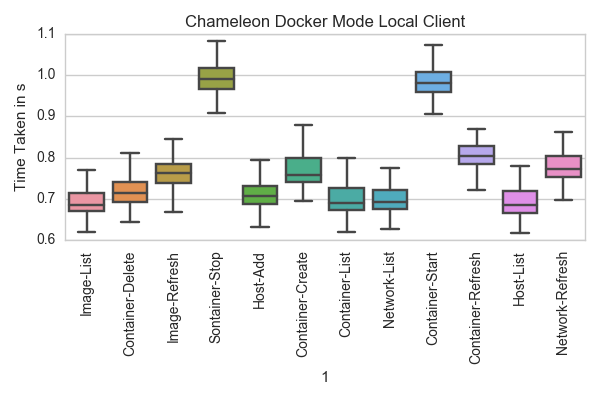
\includegraphics[width=0.8\linewidth]{images/Chameleon-Docker-Mode-Local-Client.png}}
\caption{Chameleon Docker Mode Local Client}
\label{fig:Chameleon-Docker-Mode-Local-Client}
\end{figure}


\begin{figure}[ht]
\centering
\fbox{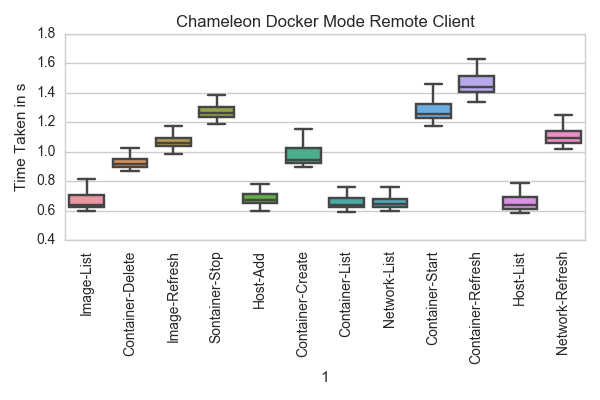
\includegraphics[width=0.8\linewidth]{images/Chameleon-Docker-Mode-Remote-Client.png}}
\caption{Chameleon Docker Mode Remote Client}
\label{fig:Chameleon-Docker-Mode-Remote-Client}
\end{figure}


\begin{figure}[h]
\centering
\fbox{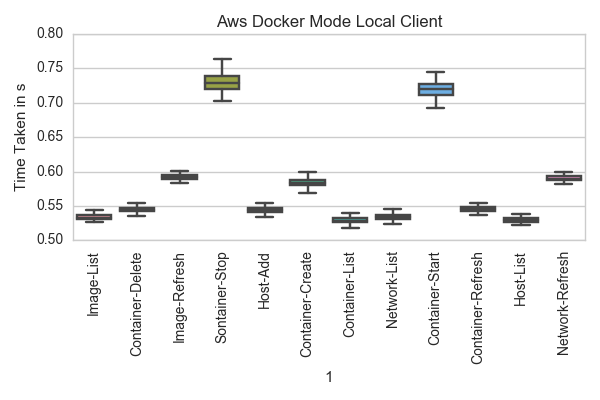
\includegraphics[width=0.8\linewidth]{images/Aws-Docker-Mode-Local-Client.png}}
\caption{Aws Docker Mode Local Client}
\label{fig:Aws-Docker-Mode-Local-Client}
\end{figure}


\begin{figure}[h]
\centering
\fbox{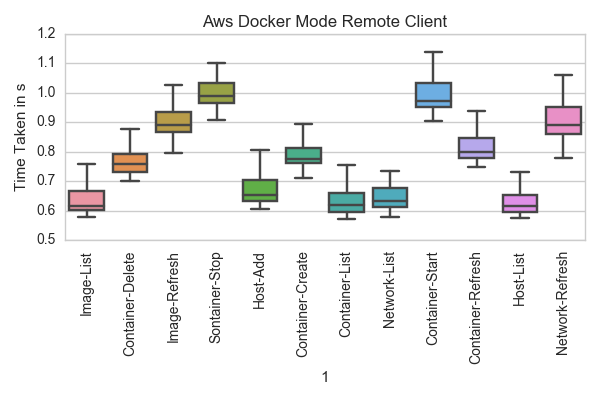
\includegraphics[width=0.8\linewidth]{images/Aws-Docker-Mode-Remote-Client.png}}
\caption{Aws Docker Mode Remote Client}
\label{fig:Aws-Docker-Mode-Remote-Client}
\end{figure}


Based on the benchmark results we can infer the below details
\begin{enumerate}
\item  In the battle of the clouds, Aws is around 20 percent faster than Chameleon cloud in docker mode
\item  Cloudmesh docker operations for the docker command performed in a local network are between
25 and 30  percent faster.We also noticed some network issues when performing the test from a
remote network, however, we chose to ignore those outliers in the plot.
\item The standard deviation of the response times is significantly lower for Aws than Chameleon indicating 
that Aws is much more stable and reliable in performance than the chameleon cloud
\item The mean container create times range between 0.5 to 1 s which is significantly faster than normal VM 
boot times on the cloud.
\end{enumerate}

\begin{table}[t]
\centering
\caption{Docker Mode AWS VS Chameleon Local Vs Remote}
\label{Docker Mode AWS VS Chameleon Local Vs Remotel}
\begin{tabular}{|l|l|l|p{0.86cm}|l|p{0.86cm}|}
\hline
 & \textbf{} & \multicolumn{2}{c|}{\textbf{Aws}} & \multicolumn{2}{c|}{\textbf{Chameleon}} \\ \hline
 & \textbf{} & \textbf{Local} & \textbf{Remote} & \textbf{Local} & \textbf{Remote} \\ \hline
\textbf{Image-List} & mean & 0.534 & 0.661 & 0.695 & 0.704 \\
\textbf{Image-List} & std & 0.004 & 0.128 & 0.039 & 0.197 \\
\textbf{Container-Delete} & mean & 0.545 & 0.785 & 0.721 & 0.951 \\
\textbf{Container-Delete} & std & 0.004 & 0.090 & 0.040 & 0.115 \\
\textbf{Image-Refresh} & mean & 0.592 & 0.925 & 0.763 & 1.139 \\
\textbf{Image-Refresh} & std & 0.005 & 0.109 & 0.040 & 0.298 \\
\textbf{Sontainer-Stop} & mean & 0.730 & 1.017 & 0.992 & 1.299 \\
\textbf{Sontainer-Stop} & std & 0.014 & 0.122 & 0.041 & 0.113 \\
\textbf{Host-Add} & mean & 0.544 & 0.691 & 0.710 & 0.727 \\
\textbf{Host-Add} & std & 0.004 & 0.114 & 0.038 & 0.194 \\
\textbf{Container-Create} & mean & 0.584 & 0.798 & 0.767 & 1.007 \\
\textbf{Container-Create} & std & 0.006 & 0.075 & 0.042 & 0.164 \\
\textbf{Container-List} & mean & 0.529 & 0.655 & 0.697 & 0.689 \\
\textbf{Container-List} & std & 0.004 & 0.110 & 0.038 & 0.141 \\
\textbf{Network-List} & mean & 0.534 & 0.668 & 0.700 & 0.679 \\
\textbf{Network-List} & std & 0.005 & 0.098 & 0.035 & 0.115 \\
\textbf{Container-Start} & mean & 0.720 & 1.018 & 0.985 & 1.310 \\
\textbf{Container-Start} & std & 0.011 & 0.145 & 0.044 & 0.169 \\
\textbf{Container-Refresh} & mean & 0.546 & 0.824 & 0.805 & 1.509 \\
\textbf{Container-Refresh} & std & 0.004 & 0.070 & 0.033 & 0.208 \\
\textbf{Host-List} & mean & 0.530 & 0.659 & 0.693 & 0.708 \\
\textbf{Host-List} & std & 0.004 & 0.125 & 0.042 & 0.273 \\
\textbf{Network-Refresh} & mean & 0.591 & 0.946 & 0.780 & 1.137 \\
\textbf{Network-Refresh} & std & 0.005 & 0.171 & 0.043 & 0.151\\
\hline
\end{tabular}
\end{table}


\subsection{Swarm Mode - Results}

Below are the categories of the Benchmark results
\begin{enumerate}
\item Chameleon Swarm Mode Local Client Figure~\ref{fig:Chameleon-Swarm-Mode-Local-Client}
\item Chameleon Swarm Mode Remote Client Figure~\ref{fig:Chameleon-Swarm-Mode-Remote-Client}
\item Aws Swarm Mode Local Client Figure~\ref{fig:Aws-Swarm-Mode-Local-Client}
\item Aws Swarm Mode Remote Client Figure~\ref{fig:Aws-Swarm-Mode-Remote-Client}
\end{enumerate}

\begin{figure}[ht]
\centering
\fbox{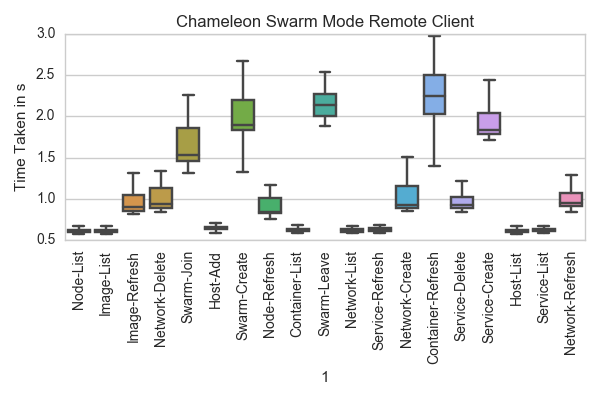
\includegraphics[width=0.8\linewidth]{images/Chameleon-Swarm-Mode-Remote-Client.png}}
\caption{Chameleon Swarm Mode Remote Client}
\label{fig:Chameleon-Swarm-Mode-Remote-Client}
\end{figure}

\begin{figure}[ht]
\centering
\fbox{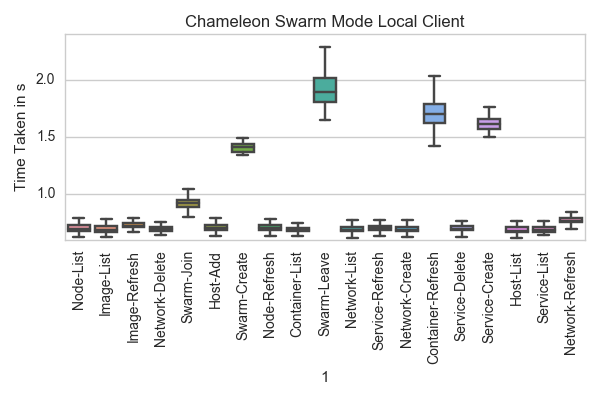
\includegraphics[width=0.8\linewidth]{images/Chameleon-Swarm-Mode-Local-Client.png}}
\caption{Chameleon Swarm Mode Local Client}
\label{fig:Chameleon-Swarm-Mode-Local-Client}
\end{figure}


\begin{figure}[h]
\centering
\fbox{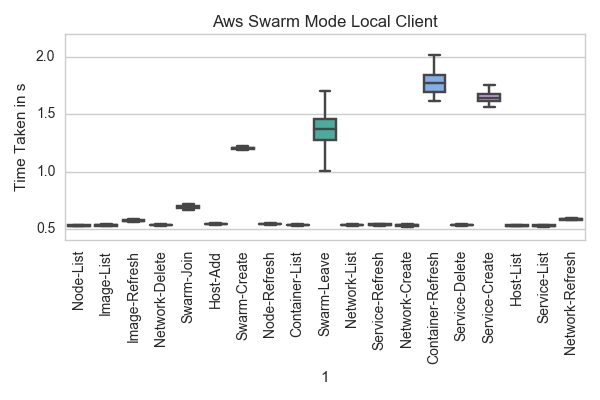
\includegraphics[width=0.8\linewidth]{images/Aws-Swarm-Mode-Local-Client.png}}
\caption{Aws Swarm Mode Local Client}
\label{fig:Aws-Swarm-Mode-Local-Client}
\end{figure}


\begin{figure}[h]
\centering
\fbox{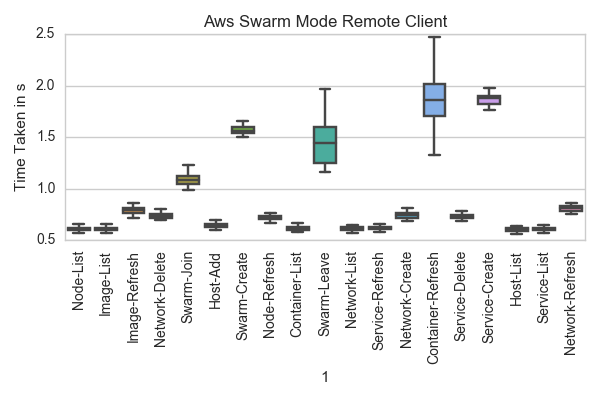
\includegraphics[width=0.8\linewidth]{images/Aws-Swarm-Mode-Remote-Client.png}}
\caption{Aws Swarm Mode Remote Client}
\label{fig:Aws-Swarm-Mode-Remote-Client}
\end{figure}

Based on the benchmark results we can infer the below details
\begin{enumerate}
\item  In the battle of the clouds, Aws is around 20 percent faster than Chameleon cloud in swarm mode
\item  Cloudmesh swarm operations for the swarm command performed in a local network are between
25 and 30  percent faster.
\item The standard deviation of the response times is significantly lower for Aws than Chameleon indicating 
that Aws is much more stable and reliable in performance than the chameleon cloud
\item The mean service create times range between 2 to 1.6 s for four replicated containers 
which is significantly faster than normal boot times for a similar number of VM on the same cloud.
\end{enumerate}

\begin{table}[t]
\centering
\caption{Swarm Mode AWS VS Chameleon Local Vs Remote}
\label{Swarm Mode AWS VS Chameleon Local Vs Remote}
\begin{tabular}{|l|l|l|p{.86cm}|l|p{0.86cm}|}
\hline
 &  & \multicolumn{2}{c|}{\textbf{Aws}} & \multicolumn{2}{l|}{\textbf{Chameleon}} \\ \hline
 &  & \textbf{Local} & \textbf{Remote} & \textbf{Local} & \textbf{Remote} \\ \hline
\textbf{Node-List} & mean & 0.529 & 0.612 & 0.704 & 0.631 \\
\textbf{Node-List} & std & 0.004 & 0.022 & 0.037 & 0.056 \\
\textbf{Image-List} & mean & 0.532 & 0.614 & 0.696 & 0.626 \\
\textbf{Image-List} & std & 0.004 & 0.041 & 0.039 & 0.053 \\
\textbf{Image-Refresh} & mean & 0.571 & 0.818 & 0.732 & 0.981 \\
\textbf{Image-Refresh} & std & 0.006 & 0.139 & 0.035 & 0.220 \\
\textbf{Network-Delete} & mean & 0.536 & 0.822 & 0.701 & 1.024 \\
\textbf{Network-Delete} & std & 0.005 & 0.280 & 0.035 & 0.247 \\
\textbf{Swarm-Join} & mean & 0.690 & 1.178 & 0.925 & 1.666 \\
\textbf{Swarm-Join} & std & 0.015 & 0.345 & 0.053 & 0.270 \\
\textbf{Host-Add} & mean & 0.542 & 0.653 & 0.714 & 0.665 \\
\textbf{Host-Add} & std & 0.005 & 0.062 & 0.035 & 0.076 \\
\textbf{Swarm-Create} & mean & 1.201 & 1.640 & 1.320 & 1.963 \\
\textbf{Swarm-Create} & std & 0.046 & 0.342 & 0.213 & 0.340 \\
\textbf{Node-Refresh} & mean & 0.542 & 0.738 & 0.714 & 0.911 \\
\textbf{Node-Refresh} & std & 0.004 & 0.107 & 0.039 & 0.127 \\
\textbf{Container-List} & mean & 0.533 & 0.622 & 0.696 & 0.638 \\
\textbf{Container-List} & std & 0.004 & 0.039 & 0.033 & 0.050 \\
\textbf{Swarm-Leave} & mean & 1.419 & 1.460 & 1.932 & 2.143 \\
\textbf{Swarm-Leave} & std & 0.275 & 0.288 & 0.241 & 0.186 \\
\textbf{Network-List} & mean & 0.532 & 0.625 & 0.698 & 0.625 \\
\textbf{Network-List} & std & 0.004 & 0.050 & 0.035 & 0.027 \\
\textbf{Service-Refresh} & mean & 0.536 & 0.631 & 0.710 & 0.645 \\
\textbf{Service-Refresh} & std & 0.004 & 0.089 & 0.039 & 0.099 \\
\textbf{Network-Create} & mean & 0.531 & 0.781 & 0.698 & 1.009 \\
\textbf{Network-Create} & std & 0.005 & 0.156 & 0.035 & 0.162 \\
\textbf{Container-Refresh} & mean & 1.666 & 1.846 & 1.693 & 2.273 \\
\textbf{Container-Refresh} & std & 0.374 & 0.348 & 0.181 & 0.386 \\
\textbf{Service-Delete} & mean & 0.535 & 0.781 & 0.704 & 0.991 \\
\textbf{Service-Delete} & std & 0.004 & 0.205 & 0.039 & 0.140 \\
\textbf{Service-Create} & mean & 1.661 & 1.905 & 1.636 & 1.938 \\
\textbf{Service-Create} & std & 0.071 & 0.164 & 0.115 & 0.273 \\
\textbf{Host-List} & mean & 0.529 & 0.608 & 0.693 & 0.629 \\
\textbf{Host-List} & std & 0.004 & 0.030 & 0.033 & 0.083 \\
\textbf{Service-List} & mean & 0.528 & 0.617 & 0.698 & 0.639 \\
\textbf{Service-List} & std & 0.005 & 0.052 & 0.035 & 0.075 \\
\textbf{Network-Refresh} & mean & 0.583 & 0.834 & 0.776 & 1.009 \\
\textbf{Network-Refresh} & std & 0.005 & 0.145 & 0.039 & 0.126\\
\hline
\end{tabular}
\end{table}

\clearpage
\section{Conclusion}

In this project, we have successfully integrated docker and swarm capabilities into the cloudmesh client.We have also demonstrated its use for a practical use case of
Setting up an Elastic search cluster in Docker and swarm modes.We have also benchmarked the commands for multiple clouds(AWS and Chameleon) in both local and remote modes and detailed the results and insights.The Ansible scripts
as part of the project along with the capabilities built in the cloudmesh docker 
application provide for a seamless capability in deploying and provisioning applications
in Docker and swarm containers.


\section{Acknowledgement}

We acknowledge our professor Gregor von Laszewski and all associate instructors for helping us and guiding us throughout this project.

\section{Appendices}
\subsection{Appendix A: Work Distribution}
The co-authors of this report worked together on the design of the technical
Solutions, implementation, testing and documentation. Below given is the work
 distribution
\begin{itemize}
\item Karthick Venkatesan
    \begin{itemize}
    \item Design and Implementation of Docker and Swarm Commands.
    \item Integration of Docker and Swarm Commands to Docker API.
    \item Integration to cloudmesh.common,cloudmesh.rest,\\
cloudmesh.cmd5 repositories.
    \item Framework definition and wrapper class built for Python-eve
    \item Ansible scripts for Docker image installation  and setup of etc hosts
    \item Test scripts for Docker and Swarm command
    \item Dockerfile for installation of cloudmesh.docker
    \item Create Benchmark scripts for Local and Remote Benchmarking on Chameleon and AWS
    \item Execute Benchmark scripts for Chameleon and Aws and plot the results in Ipython
    \item Scripts for setup of Elasticsearch Docker cluster
    \item Benchmark Elastic search swarm  cluster using ESRally and document results
    \item Writing related sections in this report.
    \end{itemize}

\item Ashok Vuppuda
    \begin{itemize}
    \item Design of Docker and Swarm Commands.
    \item Integration into cloudmesh.rest
    \item Python-eve integration and implementation for Docker and Swarm Modes
    \item Ansible scripts for Docker installation
    \item Test application on Aws and Chameleon clouds
    \item Execute Benchmark scripts for Chameleon and Aws and plot the results in Ipython
    \item Benchmark Elastic search Docker  cluster using ESRally and document results
    \item Writing related sections in this report.
    \end{itemize}
\end{itemize}


% Bibliography


\bibliography{references}
 


\newpage

\appendix


\end{document}
